\section{Mathematical Modelling, Nominal Control}

\subsection{Manipulator Dynamics}

Figure~\ref{fig_robot_kinematic} depicts the kinematic abstraction of a serial manipulator with $n$ revolute joints.

\begin{figure}[!t]
\centering
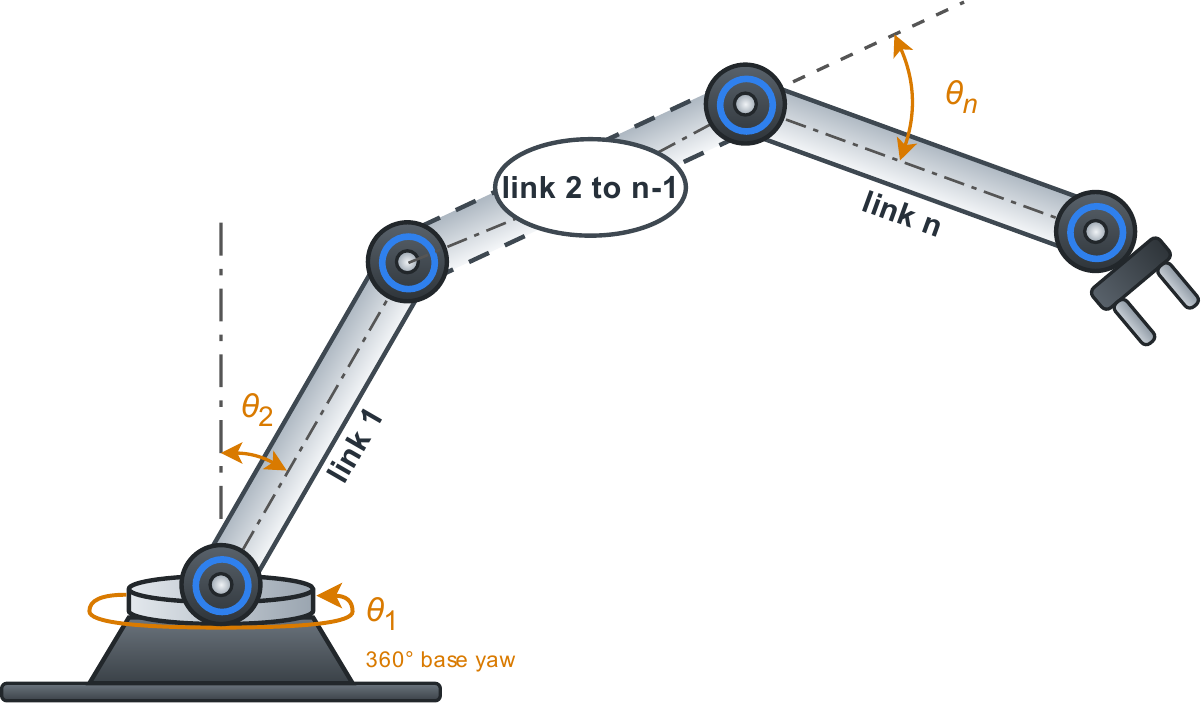
\includegraphics[width=0.7\columnwidth]{fig/robotfig-crop.png}
\caption{Kinematic abstraction of an $n$-DOF serial manipulator.}
\label{fig_robot_kinematic}
\end{figure}

For an $n$-joint manipulator, $\bm q,\dot{\bm q},\ddot{\bm q},\bm\tau,\bm d\in\R^n$ denote joint position, velocity, acceleration, applied torque, and disturbance. Its dynamics are
\begin{equation}
\bm M(\bm q)\ddot{\bm q}+\bm C(\bm q,\dot{\bm q})\dot{\bm q}
+\bm g(\bm q)+\bm F(\dot{\bm q})=\bm\tau+\bm d.
\label{eq_dynamics}
\end{equation}

Here $\bm M(\bm q),\bm C(\bm q,\dot{\bm q})\in\R^{n\times n}$, while $\bm g(\bm q),\bm F(\dot{\bm q})\in\R^n$. Define $\mathrm{ID}(\bm q,\dot{\bm q},\ddot{\bm q})=\bm M(\bm q)\ddot{\bm q}+\bm C(\bm q,\dot{\bm q})\dot{\bm q}+\bm g(\bm q)+\bm F(\dot{\bm q})$. The standard manipulator properties \cite{r18} are stated below.

\noindent\textbf{Property 1.} $\bm M(\bm q)=\bm M(\bm q)^\top\succ\bm0$. On a compact set $\mathcal Q$, constants $0<m_1\le m_2$ satisfy
\begin{equation}
m_1\bm I\preceq\bm M(\bm q)\preceq m_2\bm I,
\qquad \bm q\in\mathcal Q.
\label{eq_inertia_property}
\end{equation}

\noindent\textbf{Property 2.} For Christoffel-form $\bm C(\bm q,\dot{\bm q})$, $\dot{\bm M}(\bm q)-2\bm C(\bm q,\dot{\bm q})$ is skew-symmetric, hence
\begin{equation}
\dot{\bm M}(\bm q)=\bm C(\bm q,\dot{\bm q})+\bm C(\bm q,\dot{\bm q})^\top.
\label{eq_skew_property}
\end{equation}

The end-effector position $\bm f(\bm q)\in\R^3$ has Jacobian $\bm J_v\in\R^{3\times n}$.

\noindent\textbf{Assumption 1.} The compact set $\mathcal Q$ contains the closed joint-limit box in its interior. The model functions are continuously differentiable on an open neighborhood of the domains used below, and the position and manipulability barriers are three times continuously differentiable. Each disturbance component is absolutely continuous with $|d_i|\le\bar d_i$, $|\dot d_i|\le\bar d_{1,i}$ almost everywhere, and $|\tilde d_i(t_0)|\le\varpi_{i0}$.

\subsection{Disturbance Observer and Tracking Law}

Using generalized momentum $\bm p=\bm M(\bm q)\dot{\bm q}$ and applied torque $\bm\tau=\bm\tau^*$, Property 2 gives
\begin{equation}
\dot{\bm p}=\bm\tau^*+\bm d+\bm C(\bm q,\dot{\bm q})^\top\dot{\bm q}-\bm g(\bm q)-\bm F(\dot{\bm q}).
\label{eq_momentum}
\end{equation}

The generalized momentum observer \cite{r17} is
\begin{equation}
\begin{aligned}
\hat{\bm d}&=\bm z+\bm K_o\bm p,\\
\dot{\bm z}&=-\bm K_o(\hat{\bm d}+\bm\tau^*
+\bm C(\bm q,\dot{\bm q})^\top\dot{\bm q}-\bm g(\bm q)-\bm F(\dot{\bm q})),
\end{aligned}
\label{eq_observer}
\end{equation}

where $\bm K_o=\operatorname{diag}(k_i)\succ0$. For $\tilde{\bm d}=\bm d-\hat{\bm d}$, \eqref{eq_momentum} and \eqref{eq_observer} give $\dot{\hat{\bm d}}=\bm K_o\tilde{\bm d}$, hence $\dot{\tilde{\bm d}}=-\bm K_o\tilde{\bm d}+\dot{\bm d}$ \cite{r17}. Similar to the observer bounds in \cite{r9,r10}, this gives the mode-independent envelope
\begin{equation}
|\tilde d_i(t)|\le\varpi_i(t)=e^{-k_i(t-t_0)}\varpi_{i0}
+\frac{\bar d_{1,i}}{k_i}(1-e^{-k_i(t-t_0)}).
\label{eq_obs_envelope}
\end{equation}

For a planned motion $\bm q_p$, define $\bm e=\bm q_p-\bm q$, $\bm s=\dot{\bm e}+\bm\Lambda\bm e$, $\dot{\bm q}_r=\dot{\bm q}_p+\bm\Lambda\bm e$, and $\ddot{\bm q}_r=\ddot{\bm q}_p+\bm\Lambda\dot{\bm e}$, where $\bm\Lambda=\operatorname{diag}(\lambda_i)\succ0$. The Slotine-Li-type controller \cite{r18}, here with inertia-scaled damping, is
\begin{equation}
\begin{aligned}
\bm u_{\rm nom}={}&\bm M(\bm q)\ddot{\bm q}_r
+\bm C(\bm q,\dot{\bm q})\dot{\bm q}_r\\
&+\bm g(\bm q)+\bm F(\dot{\bm q})\\
&+\kappa\bm M(\bm q)\bm s-\hat{\bm d},\quad\kappa>0.
\end{aligned}
\label{eq_controller}
\end{equation}

For $\Delta\bm\tau=\bm\tau^*-\bm u_{\rm nom}$, the tracking dynamics become
\begin{equation}
\bm M(\bm q)\dot{\bm s}+(\bm C(\bm q,\dot{\bm q})+\kappa\bm M(\bm q))\bm s
=-\tilde{\bm d}-\Delta\bm\tau.
\label{eq_tracking}
\end{equation}

\subsection{Stability Analysis of the Slotine-Li Controller}

\begin{theorem}
Under Properties 1-2 and Assumption 1, let
$y=\sqrt{\bm s^\top\bm M(\bm q)\bm s}$.
While $\bm q\in\mathcal Q$, the tracking dynamics
\eqref{eq_tracking} satisfy
\begin{equation}
\begin{aligned}
y(t)\le{}&e^{-\kappa(t-t_0)}y(t_0)\\
&+\frac{1}{\sqrt{m_1}}\int_{t_0}^{t}
e^{-\kappa(t-\sigma)}
(\|\tilde{\bm d}\|+\|\Delta\bm\tau\|)\,d\sigma.
\end{aligned}
\label{eq_iss}
\end{equation}

Thus, tracking is input-to-state stable, with
exponential convergence when both perturbations vanish.
\end{theorem}

\begin{proof}
Choose $V=\tfrac12\bm s^\top\bm M(\bm q)\bm s$.
By Property 2 and \eqref{eq_tracking},
\begin{equation}
\dot V=-\kappa\bm s^\top\bm M(\bm q)\bm s
-\bm s^\top(\tilde{\bm d}+\Delta\bm\tau).
\label{eq_slotine_lyap}
\end{equation}

The inertia-weighted Cauchy-Schwarz inequality gives
$D^+y\le-\kappa y+
\|\bm M(\bm q)^{-1/2}(\tilde{\bm d}+\Delta\bm\tau)\|$,
including the upper right Dini derivative at $y=0$.
Property 1 then gives
$D^+y\le-\kappa y+
(\|\tilde{\bm d}\|+\|\Delta\bm\tau\|)/\sqrt{m_1}$.
Scalar comparison proves \eqref{eq_iss}.
Since $\dot{\bm e}=-\bm\Lambda\bm e+\bm s$,
vanishing perturbations imply exponential
convergence of $\bm e$ and $\dot{\bm e}$.
\end{proof}

\subsection{Robust HOCBF-QP Filter}

Define the joint-position barriers
$h_{i,+}=q_{\max,i}-q_i$,
$h_{i,-}=q_i-q_{\min,i}$, the manipulability
barrier
$h_{\rm man}=\det(\bm J_v\bm J_v^\top)-w_{\min}^2$
\cite{r6,r14}, and velocity barriers
$h_{v,i,\pm}=\dot q_{\max,i}\mp\dot q_i$.
For each position-level barrier $h_j$, imposed at the acceleration level, the HOCBF condition \cite{r8} is
\begin{equation}
\begin{aligned}
\mathcal H_j={}&
\nabla h_j^\top\ddot{\bm q}
+\dot{\bm q}^\top\nabla^2h_j\dot{\bm q}\\
&+(\alpha_1+\alpha_2)\nabla h_j^\top\dot{\bm q}
+\alpha_1\alpha_2h_j,
\end{aligned}
\label{eq_hocbf}
\end{equation}

where $\alpha_1,\alpha_2>0$.
Using the estimated acceleration
\begin{equation}
\ddot{\hat{\bm q}}(\bm\tau)
=\bm M(\bm q)^{-1}
[\bm\tau+\hat{\bm d}
-\mathrm{ID}(\bm q,\dot{\bm q},\bm0)],
\end{equation}

define
$A_{jl}=[\nabla h_j^\top\bm M(\bm q)^{-1}]_l$
and $N_{il}=[\bm M(\bm q)^{-1}]_{il}$.
The robust CBF constraints \cite{r9,r10,r11} are
\begin{equation}
\begin{aligned}
\Psi_j(\bm\tau)&=
\mathcal H_j(\bm q,\dot{\bm q},
\ddot{\hat{\bm q}}(\bm\tau))
-\sum_l|A_{jl}|\varpi_l,\\
\Xi_{i,\pm}(\bm\tau)&=
\mp\ddot{\hat q}_i(\bm\tau)
+\alpha_vh_{v,i,\pm}
-\sum_l|N_{il}|\varpi_l,
\end{aligned}
\label{eq_robust_cbf}
\end{equation}
The safety filter solves
\begin{equation}
\begin{aligned}
\bm\tau^*=\arg\min_{\bm\tau}\quad&
\tfrac12\|\bm\tau-\bm u_{\rm nom}\|^2\\
\mathrm{s.t.}\quad&
\Psi_j(\bm\tau)\ge0,\quad
\Xi_{i,\pm}(\bm\tau)\ge0,\\
&|\tau_i|\le\tau_{\max,i}.
\end{aligned}
\label{eq_hard_qp}
\end{equation}
When \eqref{eq_hard_qp} is infeasible, $\bm\tau^*$ denotes the recovery torque of Section~\ref{subsec_recovery}, so \eqref{eq_observer} always uses the applied torque.
